DARWIN is a new method and according to knowledge of the author and the
supervisor haven't been implemented before. Experiments are
designed to check if the method is working at all, what parameters are important
for the method and what should be their reasonable default values. To make
results repeatable the DM is mocked. Noise in his or her decisions is
simulated. Unless uncertainty is involved comparisons to exact optimal
solution are provided. In tests involving uncertainty results are compared to
supposed utility function optimisation. 

\section{The environment}

All tests were conducted on a personal computer with 64bit Intel
processor. RAM size on the machine is 3GB. 64bit Linux operating system was
used. The Java Virtual Machine was in version 1.6.0\_18 and Scala 2.8.0. JVM
was run with options \texttt{-Xms768m -Xmx768m} thus setting memory available
for application to 768MB. Tests were performed through CLI batch interface.

Test framework is available in order to automate the experiment process. All
experiments were repeated at least thirteen times. Data analysis and chart
generation was performed using an R environment [ref]. The framework is a
combination of Python [ref] and Bash [ref] code communicating with main DARWIN
code and with the modules written in R.

\section{The Decision Maker}

Experiments were repeated many times. In order to make it possible it was
essential to mock the DM. This was also done to assure repeatable process
across the test runs.

In the DARWIN method interaction with decision maker occurs by showing him or
her a list of generated solutions (usually 30) and asking him or her to
indicate few ``good'' ones.

To mock the DM one need to simulate his or her selections. It is assumed that
the decision maker acts according to a utility functions he or her has in
mind. This function will be called the supposed utility function.

In the mocking process algorithm sorts the received solutions list according
to this supposed utility function. Then it selects three (usually three,
however this can be configured) solutions with the highest supposed utility.

Unfortunately real decision maker, being a human isn't a predictive and
repeatable as the described process. In the section [inref] results of
introducing noise to DM's decisions are presented.

In the following problems the supposed utility function is also defined.

\section{Problem selection}

Area of interest for Multi-Objective Optimisation is huge and consists of many
potential problems to be solved. There are multi-criteria versions of
classical problems, like minimal spanning tree~[ref], traveling salesman
problem (TSP)~[ref] or knapsack problem~[ref] as well as artificially
generated ones --- like the DTLZ problems [ref]. Some of them are interesting
because of their real-life applications while the other are good for
experimenting and testing purposes.

It is worth noting that the ordinary single-criterion versions of the problems
can be easy to solve. However in multi-criteria setting one has to infer the
decision maker preferences and approximate supposed utility function
correctly. The challenge here is not to build the best optimisation algorithm
for all the problems (what is impossible according to no-free-lunch theorem
[ref]) but rather a framework for preference information extraction.

Introducing uncertainty model as intervals is a new concept. For this reason
the uncertainty was added to the problems described above.

The experiments were performed using following problems:
\begin{description}
  \item{\textbf{Two-criteria binary knapsack problem}}
    \begin{align*}
      & \bar{x} = [x_1, x_2, \dots, x_{300}]  \\
      & x_i \in \{0, 1\};  \hspace{0.5cm} i = 1, 2, \dots, 300 \\
      & \textit{max}\text{ value$_1$:} \hspace{0.2cm} \bar{a_1} \cdot \bar{x} \\
      & \textit{max}\text{ value$_2$:} \hspace{0.2cm} \bar{a_2} \cdot \bar{x} \\
      & \textit{subject to:} \\
      & \hspace{0.5cm} \text{weight:} \hspace{0.2cm} \bar{w} \cdot \bar{x}
      \leq b \\
      & \textit{(max) supposed utility:} \\
      & \hspace{0.5cm} 1*\text{value}_1 + 2*\text{value}_2
    \end{align*}
    
    Where $\bar{x}$ is a vector of items to be chosen. The problem is binary,
    so each $x_i \in \bar{x}$ can be either selected ($x_i = 1$) or not($x_i
    = 0$). There are two criteria: value$_1$ and value$_2$. Each one is a sum
    of items multiplied with associated weights (vector $\bar{a_1}$ and
    $\bar{a_2}$).

    Knapsack constraint is given. One can choose items up to a certain weight
    ($b$). There is a vector of weights associated with each item
    ($\bar{w}$). The limit is defined that it is possible to choose about
    $2/3$ of the items.

    Weights ($\bar{a_1}, \bar{a_2}, \bar{w}$) are uniformly distributed
    vectors of values in $[0,10)$ interval.


  \item{\textbf{Two-criteria continuous knapsack problem}}
    \begin{align*}
      & \bar{x} = [x_1, x_2, \dots, x_{300}]  \\
      & x_i \in [0, 1);  \hspace{0.5cm} i = 1, 2, \dots, 300 \\
      & \textit{max}\text{ value$_1$:} \hspace{0.2cm} \bar{a_1} \cdot \bar{x} \\
      & \textit{max}\text{ value$_2$:} \hspace{0.2cm} \bar{a_2} \cdot \bar{x} \\
      & \textit{subject to:} \\
      & \hspace{0.5cm} \text{weight:}  \hspace{0.2cm} \bar{w} \cdot \bar{x}
        \leq b \\
      & \textit{(max) supposed utility:} \\
      & \hspace{0.5cm} 3 * \text{value}_1 - 1 * \text{value}_2
    \end{align*}

    Continuous version of the knapsack problem. Description given for the
    binary version also applies here. The only difference is that now item can
    be partially selected ($\forall_{x_i \in \bar{x}} x_i \in [0, 1)$). 

  \item{\textbf{Three-criteria binary knapsack problem}}
    \begin{align*}
      & \bar{x} = [x_1, x_2, \dots, x_{300}]  \\
      & x_i \in \{0, 1\};  \hspace{0.5cm} i = 1, 2, \dots, 300 \\
      & \textit{max}\text{ value$_1$:} \hspace{0.2cm} \bar{a_1} \cdot \bar{x} \\
      & \textit{max}\text{ value$_2$:} \hspace{0.2cm} \bar{a_2} \cdot \bar{x} \\
      & \textit{max}\text{ value$_3$:} \hspace{0.2cm} \bar{a_3} \cdot \bar{x} \\
      & \textit{subject to:} \\
      & \hspace{0.5cm} \text{weight:} \hspace{0.2cm} \bar{w} \cdot \bar{x}
      \leq b \\
      & \textit{(max) supposed utility:} \\
      & \hspace{0.5cm} 1 * \text{value}_1 - 1 * \text{value}_2 + 2 * \text{value}_22
    \end{align*}

    Two-criteria problems can be easily visualised and analysed, however in
    real-life applications there is often a need for three and more
    criteria. There is a moving from two to multiple, so it is worth comparing
    the results achieved on the three-criteria knapsack problem with its
    two-criteria counterpart. 

  \item{\textbf{Three-criteria DTLZ problem generated using constraint surface
    approach}}
    \begin{align*}
      & \textit{min}\text{ f$_1$:} \hspace{0.2cm} x_1 \\
      & \textit{min}\text{ f$_2$:} \hspace{0.2cm} x_2 \\
      & \textit{min}\text{ f$_3$:} \hspace{0.2cm} x_3 \\
      & \textit{subject to:} \\
      & \hspace{0.5cm} 0 \le x_i \le 1, \hspace{0.2cm} i = 1, 2, 3 \\
      & \hspace{0.5cm} -x_1 + x_2 + 0.6 \ge 0 \\
      & \hspace{0.5cm} x_1 + x_3 - 0.5 \ge 0 \\
      & \hspace{0.5cm} x_1 + x_2 + x_3 - 1.1 \ge 0 \\
      & \textit{(max) supposed utility:} \\
      & \hspace{0.5cm} -1 * \text{f}_1 - 2 * \text{f}_2 - 1 * \text{f}_3
    \end{align*}

    This problem consists of three simple linear criteria. The solution space
    is three dimensional cube bounded by the $0 \le x_i \le 1$ constraint. To
    make the problem more interesting parts of the solution space are being
    cut off by additional constraints.

    This problem was build according to constraint surface approach presented
    in~[ref].

  \item{\textbf{Two-criteria robust mix problem}}
    \begin{align*}
      & \textit{max}\text{ profit:} \hspace{0.2cm} p_A \text{min}(x_A, d_A)
      + p_B \text{min}(x_B, d_B) +  p_C \text{min}(x_C, d_C) \\
      & \hspace{1cm} - (r^1_Ax_A + r^1_Bx_B + r^1_Cx_C) p^1_R
      - (r^2_Ax_A + r^2_Bx_B + r^2_Cx_C) p^2_R\\
      & \textit{min}\text{ time:} \hspace{0.2cm} t_Ax_A + t_Bx_B + t_Cx_C \\
      & \textit{where:} \\
      & \hspace{0.5cm} p_A \in [20, 24], p_B \in [30, 36], p_C \in [25, 30] \\
      & \hspace{0.5cm} d_A \in [10, 12], d_B \in [20, 24], d_C \in [10, 12] \\
      & \hspace{0.5cm} r^1_A \in [1, 1.2], r^1_B \in [2, 2.4], r^1_C \in [0.75, 0.9] \\ 
      & \hspace{0.5cm} r^2_A \in [0,5, 0.6], r^2_B \in [1, 1.2], r^2_C \in [0.5, 0.6] \\ 
      & \hspace{0.5cm} p^1_R \in [6, 7.2], p^2_R \in [9, 9.6] \\
      & \hspace{0.5cm} t_A \in [5, 6], t_B \in [8, 9.6], t_C \in [10, 12] \\ 
      & \textit{subject to:} \\
      & \hspace{0.5cm} 0 \le x_A \le 12 \\
      & \hspace{0.5cm} 0 \le x_B \le 24 \\
      & \hspace{0.5cm} 0 \le x_C \le 12 \\
      & \textit{(max) supposed utility:} \\
      & \hspace{0.5cm} \text{profit}^{1\%} + 3 * \text{profit}^{25\%}
      + 2 * \text{profit}^{50\%} - \text{time}^{1\%}
      - 3 * \text{time}^{25\%} - 2 * \text{time}^{50\%} 
    \end{align*}
    
    
    The problem was described in a presentation given on ... ([ref])
    describing the DARWIN method. It contains a lot of coefficients given in
    form of intervals. For readability's sake they were named and defined
    below the criteria.

    The goal is to decide quantity of each product ($A, B, C$) to be
    produced. One wants to maximise the profit and minimised the total time it
    takes to produce the products. $p_i$ is the price of a product $i \in \{A,
    B, C\}$ on the market. There is also maximal demand the market can consume
    ($d_i$). Each product consists of two raw materials --- $r_1$ and
    $r_2$. Quantity needed to produce $i$-th product is defined ($r^1_i,
    r^2_i$) as well as the product price ($p^1_R, p^2_R$). Finally it takes
    time to produce a given product --- $t_A, t_B, t_C$.

    Coefficients are given in form of intervals, so each solution has to be
    evaluated on many scenarios of uncertainty. This is why no exact values
    are given in the supposed utility function. Percentiles are given instead
    (see~[inref]). $\text{goal}^{25\%}$ means the best solution of the worst
    $25\%$ of them.

  \item{\textbf{Four-criteria robust DTLZ7 problem}}
    \begin{align*}
      & \textit{min}\text{ $f_j(x)$:} \hspace{0.2cm}
      0.1 * \sum_{10(j-1) + 1}^{10j}x_i + [0, 2*(4-j)], \hspace{0.2cm}
      j = 1, 2, 3, 4\\
      & \textit{subject to:} \\
      & \hspace{0.5cm} g_1(x)\text{: } f_4(x) + 4f_1(x) - 1 \ge 0\\
      & \hspace{0.5cm} g_2(x)\text{: } f_4(x) + 4f_2(x) - 1 \ge 0\\
      & \hspace{0.5cm} g_3(x)\text{: } f_4(x) + 4f_3(x) - 1 \ge 0\\
      & \hspace{0.5cm} g_3(x)\text{: } 2*f_4(x) + \text{min}
      [f_1(x) + f_2(x), f_1(x) + f_3(x), f_2(x) + f_3(x)] -1 \ge 0\\
      & \hspace{0.5cm} 0 \le x_i \le 1, \hspace{0.2cm} i = 1, 2, 3, 4 \\
      & \textit{(max) supposed utility:} \\
      & \hspace{0.5cm} -4 * \text{f}_1^{60\%} -3 * \text{f}_2^{60\%}
      -2 * \text{f}_3^{60\%} -1 * \text{f}_1^{60\%}
      -8 * \text{f}_1^{30\%} -6 * \text{f}_2^{30\%}
      -4 * \text{f}_3^{30\%} -2 * \text{f}_1^{30\%}
    \end{align*}

    This problem is a variation of DTLZ7 problem from [ref] article. The
    problem was constructed using constraint surface approach describe in the
    article. Interval coefficients were added to the goals however.


  \item{\textbf{Robust DTLZ1 problem}}
    \begin{align*}
      & \textit{min}\text{ $f_1(x)$:} \hspace{0.2cm}
      [0.3, 0.7] * x_1 x_2 \dots x_{M-1}(1 + g(x_M)) \\
      & \textit{min}\text{ $f_2(x)$:} \hspace{0.2cm}
      [0.3, 0.7] * x_1 x_2 \dots (1 - x_{M-1})(1 + g(x_M)) \\
      & \hspace{0.5cm} \dots \\
      & \textit{min}\text{ $f_{M-1}(x)$:} \hspace{0.2cm}
      [0.3, 0.7] * x_1 (1 - x_2) (1 + g(x_M)) \\
      & \textit{min}\text{ $f_M(x)$:} \hspace{0.2cm}
      [0.3, 0.7] * (1 - x_1) (1 + g(x_M)) \\
      & \textit{where:} \\ 
      & \hspace{0.5cm} g(x) = 100 * (5 + \sum_{i=M}^{M+4}
        [ (x_i - 0.5)^2 - \text{cos}(20 \pi (x_i -0.5)) ])\\
      & n = M + 4 \\
      & \textit{subject to:} \\  
      & \hspace{0.5cm} 0 \le x_i \le 1, \hspace{0.2cm} i = 1, 2, \dots n \\
      & \textit{(max) supposed utility:} \\
      & \hspace{0.5cm} \sum_{i=1}^M (-M+i-1) * f_i^{25\%} 
    \end{align*}

  Another problem suggested in [ref]. It was constructed using bottom-up
  approach ([ref]). Intervals were added to the goal functions. $M$ indicates
  number of goals. In the experiments problem with 4 an 10 criteria were used.

\end{description}

\section{No uncertainty}

\subsection{Single run analysis}
In order to observe the algorithm's behaviour a detailed analysis of single
run is presented in this section. The problem being analysed is the two
criteria binary knapsack problem (see [inref]). Problem is simple and number
of criteria small in order to focus on the algorithm. Also no uncertainty in
form of interval coefficients is considered.

Although this section is illustrated by an example run on the single problem
the conclusions drawn here applies globally. Compare with further sections of
the chapter.

The exterior loop of the DARWIN was repeated ten times. The algorithm runs
with default parameters (see [inref]). Exterior loop was repeated ten
times. This means that ten times results (in form of solutions) were presented
to the (mocked) decision maker. The solutions were recorded.

The same problem was also solved by a mathematical programming solver
(glpk~[ref]). One used supposed utility function as a optimisation goal for
the solver. This way the best solutions was obtained (for the considered
instance best supposed utility function value is $4154.441453$).

Results of the run from the exterior loop perspective are given on
figure~\ref{c2_utilouter}. All of the solutions generated during interior loop
run were recorded. On the chart one see best and worst solutions in given run
(the rest lies between them). Also best of the solutions shown to the DM is
presented (labeled as ``last''). This is because for evolutionary algorithm it
is possible to find and then forget ``good'' solutions (note that optimisation
--- the internal loop is not aware of supposed utility function, it only tries
to approximate it using induced decision rules). However most of the times
``last'' solution equals ``best'' solution.

One can see that in every iteration there is an improvement, however the
improvements are getting smaller and smaller. This is because the better the
solution population the harder it is to optimise it further.

Now analysis of the interior loop is given. The first, third and seventh
interior loop will be presented. Other runs are similar, so they were omitted
in the paper. The results are presented on figures \ref{c2_utilgen_01},
\ref{c2_utilgen_03} and \ref{c2_utilgen_07}. The iterations of the interior
loop are also called \textit{generations} because of their evolutionary
nature.

On the charts one can see supposed utility function dependent on
generation. Also value of the primary score is included for reference. To
recapitulate --- the better the solution fits to induced decision rules the
higher the primary score; in case of a draw (i.e. the primary score for two
individuals is the same) secondary score is considered.

The improvement happens on generation basis --- in every iteration supposed
utility function is getting better. However as one can see improvement of the
primary score happens mainly at the beginning. The runs like one in
\ref{c2_utilgen_07}, where the is a breakthrough at the end of the run are in
fact rare. Nevertheless the algorithm shouldn't be shut down after reaching
maximum primary score. Although preference information extracted before the
run are now exploited still an improvement can occur. More importantly the
diversification effort is ongoing now --- when the primary score (rule based)
of all the population is identical the secondary score (distance based --- the
less the solution is crowded the higher the score) start to play major role in
the process, pushing individuals in the population to new areas in solution
space. This can result in major breakthrough --- the population may acquire
traits wanted by the DM.

Rules driving the interior loops are presented below

\begin{description}
  \item{\textbf{Iteration 1}} \\
    value$_1 \ge 859.86 \Rightarrow \text{class} \ge \texttt{GOOD}$ \\
    value$_2 \ge 814.71 \Rightarrow \text{class} \ge \texttt{GOOD}$
  \item{\textbf{Iteration 3}} \\
    value$_1 \ge 1023.62 \Rightarrow \text{class} \ge \texttt{GOOD}$ \\
    value$_2 \ge 1011.61 \Rightarrow \text{class} \ge \texttt{GOOD}$
  \item{\textbf{Iteration 7}} \\
    value$_1 \ge 1211.14 \Rightarrow \text{class} \ge \texttt{GOOD}$ \\
    value$_2 \ge 1210.63 \Rightarrow \text{class} \ge \texttt{GOOD}$
\end{description}

Note that there are only two classes --- \texttt{GOOD} and \texttt{NOT GOOD}
so essentially $\text{class} \ge \texttt{GOOD}$ means $\text{class} =
\texttt{GOOD}$.

In order to verify how the rules influences the algorithm behaviour charts
were prepared (fig.~\ref{c2_valweight_01}, \ref{c2_valweight_03} and
\ref{c2_valweight_07}). For two-criteria problem it is possible to present the
search space on two-dimensional chart.

The iterations $1$ and $3$ show typical run. Before the 10th generation whole
population moves to an area covered by the rules. In the further generations
diversification occurs. 7th iteration is a bit different though. Evolution
``discovered'' a way to match the second rule not before the 20th
generation. Soon after individuals covering both solutions were included the
whole population drifted to the region marked by both rules.

It can be also insightful to see the mocked DM choices and compare them with the
inferred  rules. They are presented on charts (fig.~\ref{c2_dmchoices_01},
\ref{c2_dmchoices_03}, \ref{c2_dmchoices_07}). It is the case that the choices
directly affected the rules. One can also see another interesting trait of the
problem. The further (in goal functions' space) the selected individuals are
the harder it is to achieve maximal possible primary score.

Finally charts presenting how supposed utility and primary score changed in
the population together with succeeding generations (fig.~\ref{c2_utilind_01},
\ref{c2_utilind_03} and \ref{c2_utilind_07}) are given. They are supporting
the conclusions stated above.

Analysis of single run it a good tool for understanding the internals of the
method and inspecting the method behaviour. One can draw conclusions and spot
potential problems and possible improvements. However more experiments have to
be conducted and their results should be aggregated using statistical methods
in order to check how useful the method is and what is the influence of the
algorithm parameters. This is done in the further sections.

%% Charts
\begin{figure}[tb]
  \centering 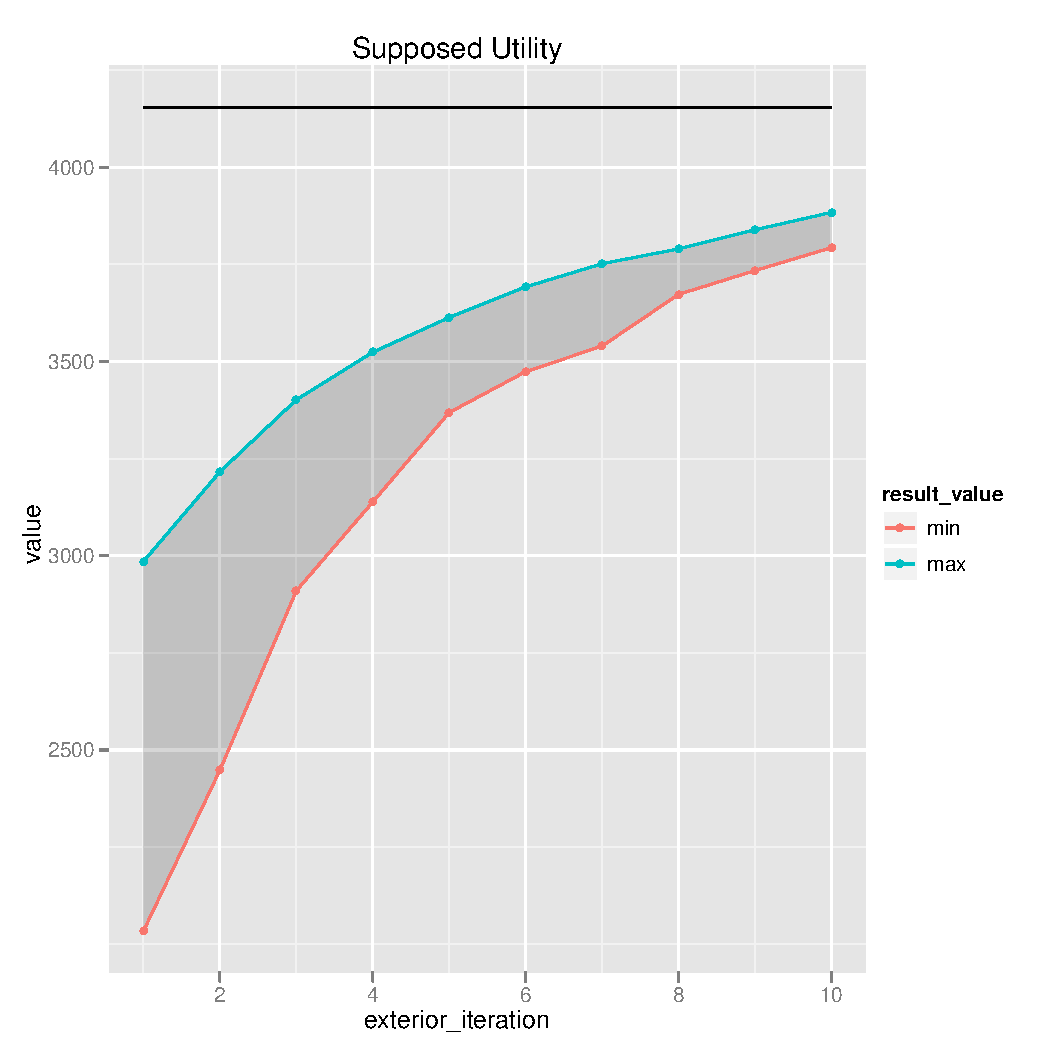
\includegraphics[width=1.0\textwidth]{exp/nouncert/c2_utilouter}
  \caption{Supposed utility function in exterior loop iterations}
  \label{c2_utilouter}
\end{figure}


%% Utilgen
\begin{figure}
  \centering 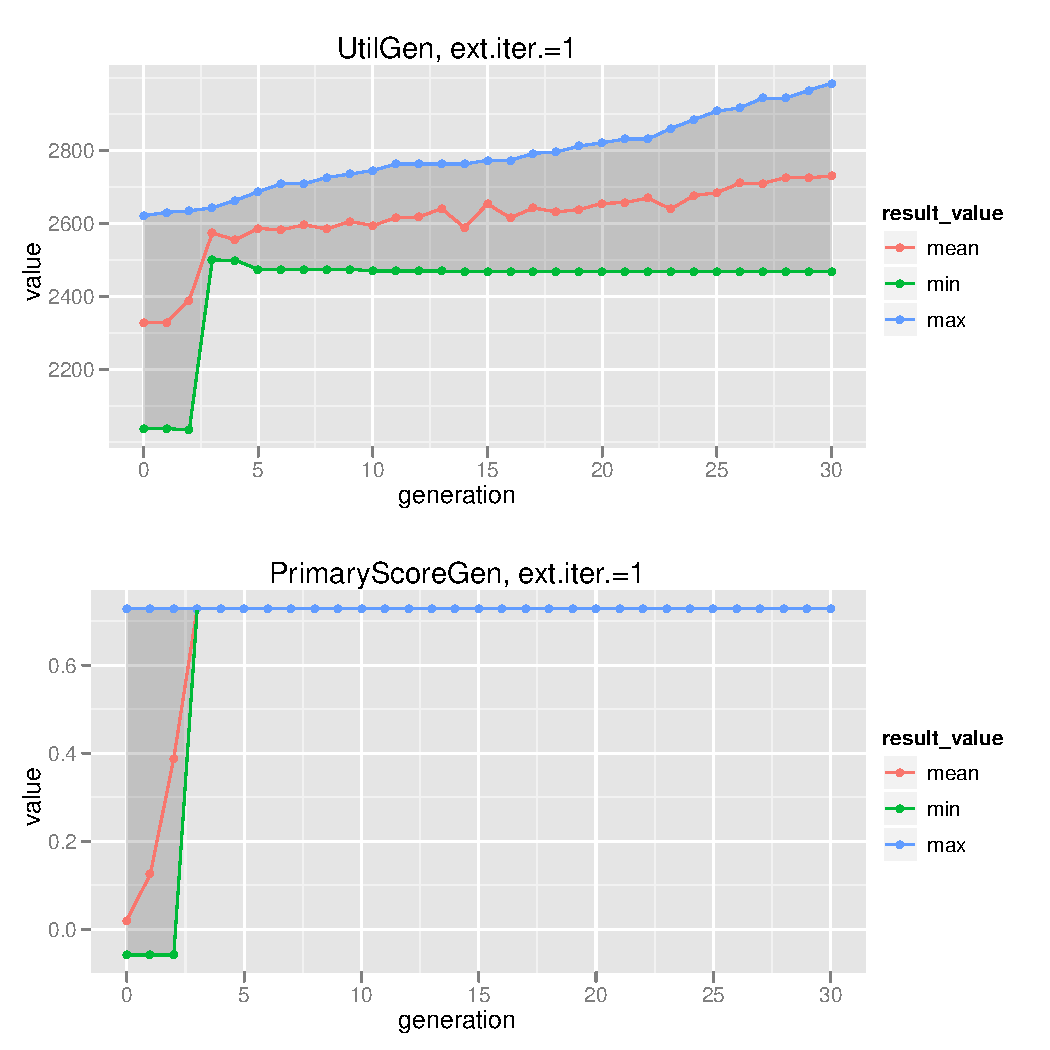
\includegraphics[width=1.0\textwidth]{exp/nouncert/c2_utilgen_01}
  \caption{Supposed utility function in interior loop iterations}
  \label{c2_utilgen_01}
\end{figure}

\begin{figure}
  \centering 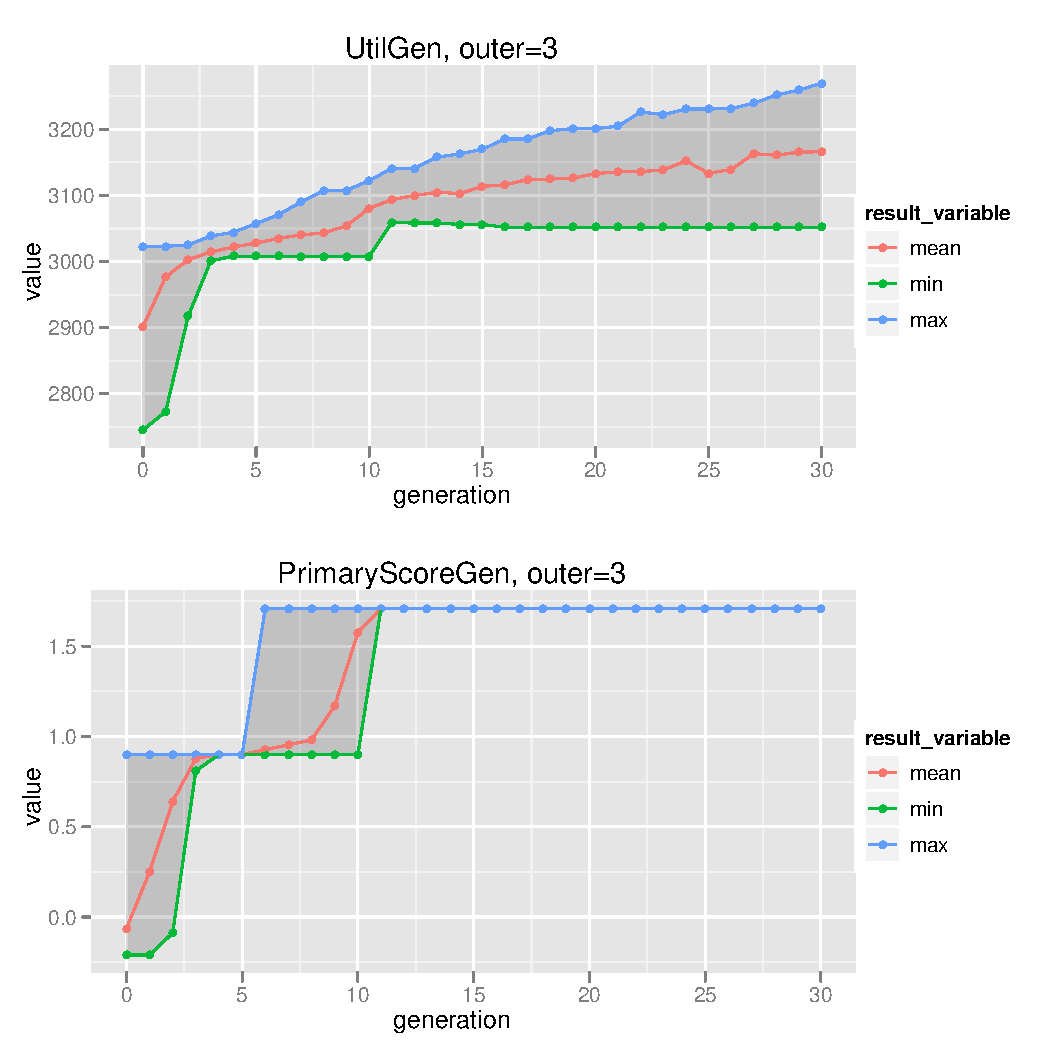
\includegraphics[width=1.0\textwidth]{exp/nouncert/c2_utilgen_03}
  \caption{Supposed utility function in interior loop iterations}
  \label{c2_utilgen_03}
\end{figure}

\begin{figure}
  \centering 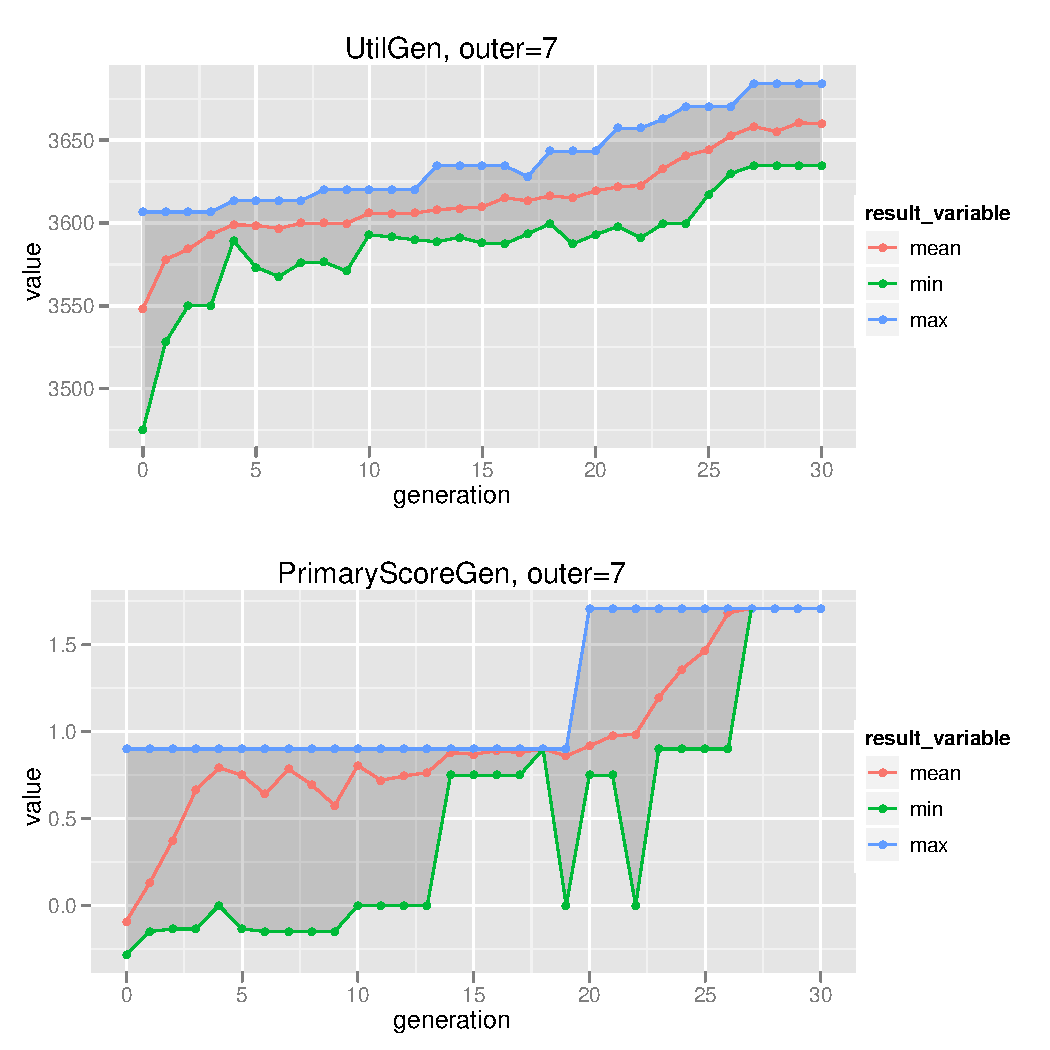
\includegraphics[width=1.0\textwidth]{exp/nouncert/c2_utilgen_07}
  \caption{Supposed utility function in interior loop iterations}
  \label{c2_utilgen_07}
\end{figure}

%% Valweight
\begin{figure}
  \subfigure{
    \hspace*{-3.3cm}
    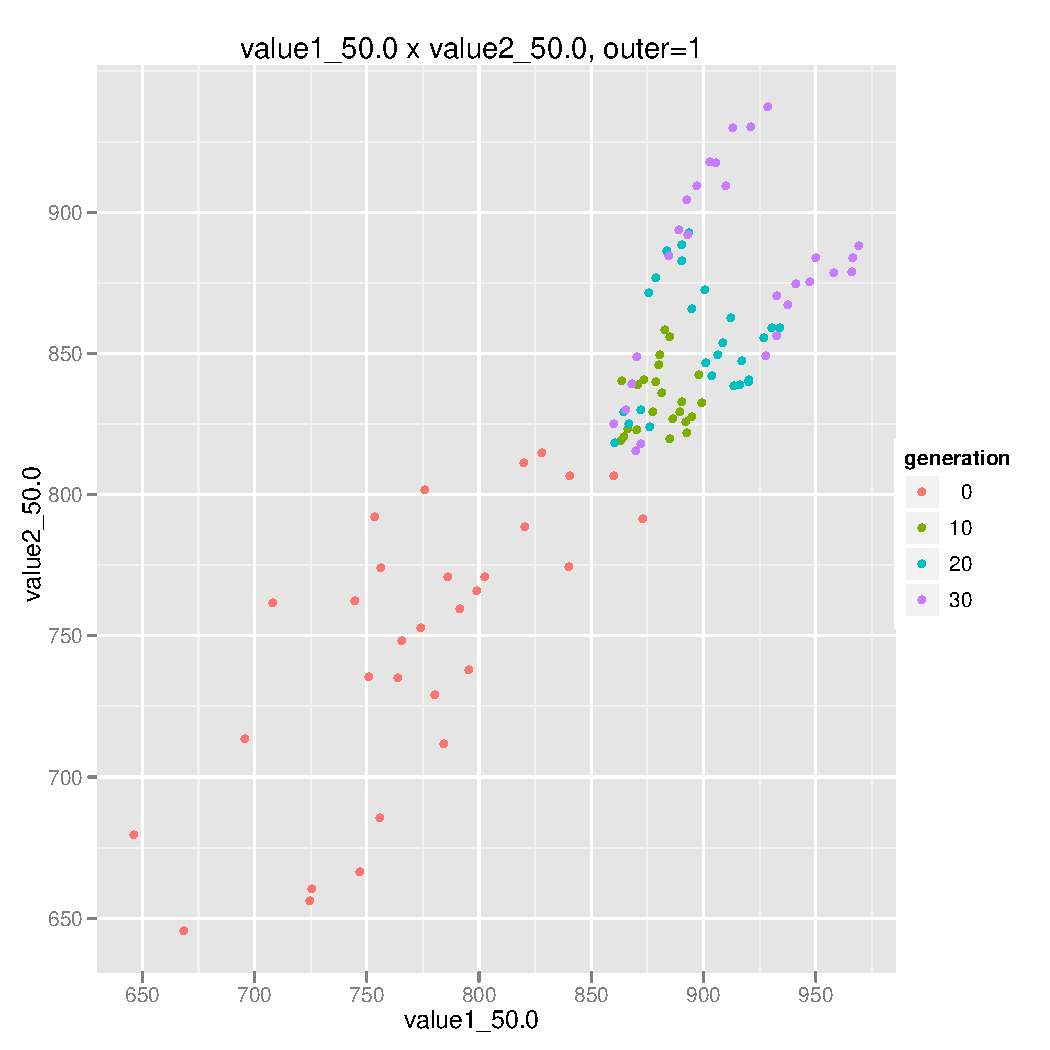
\includegraphics[scale=0.57]{exp/nouncert/c2_valweight_01}
    \label{c2_valweight_01}
  }
  \subfigure{
    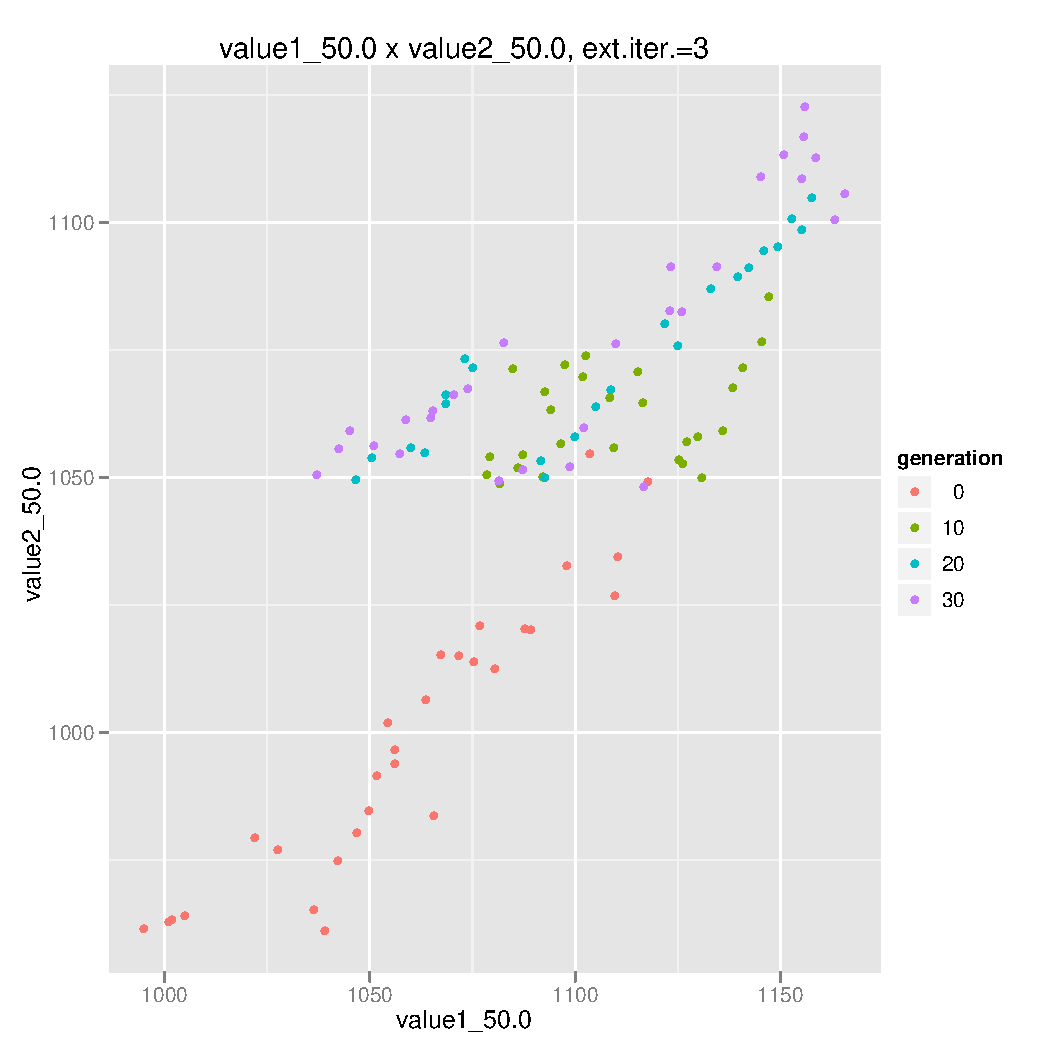
\includegraphics[scale=0.57]{exp/nouncert/c2_valweight_03}
    \label{c2_valweight_03}
  }
  \subfigure{
    \hspace*{2cm}
    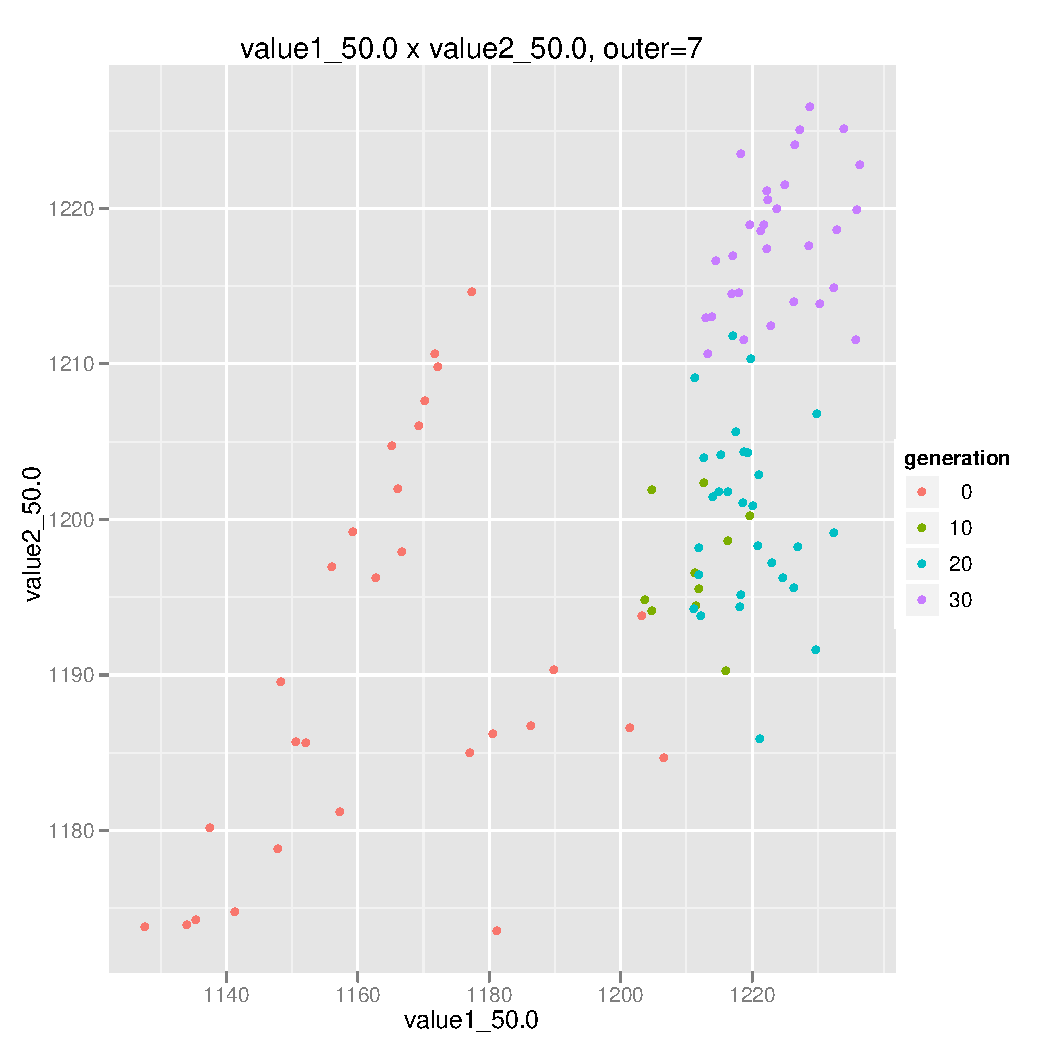
\includegraphics[scale=0.57]{exp/nouncert/c2_valweight_07}
    \label{c2_valweight_07}
  }
  \caption{Individuals in the solution space}
\end{figure}


%% DM's choices
\begin{figure}
  \subfigure{
    \hspace*{-2.5cm}
    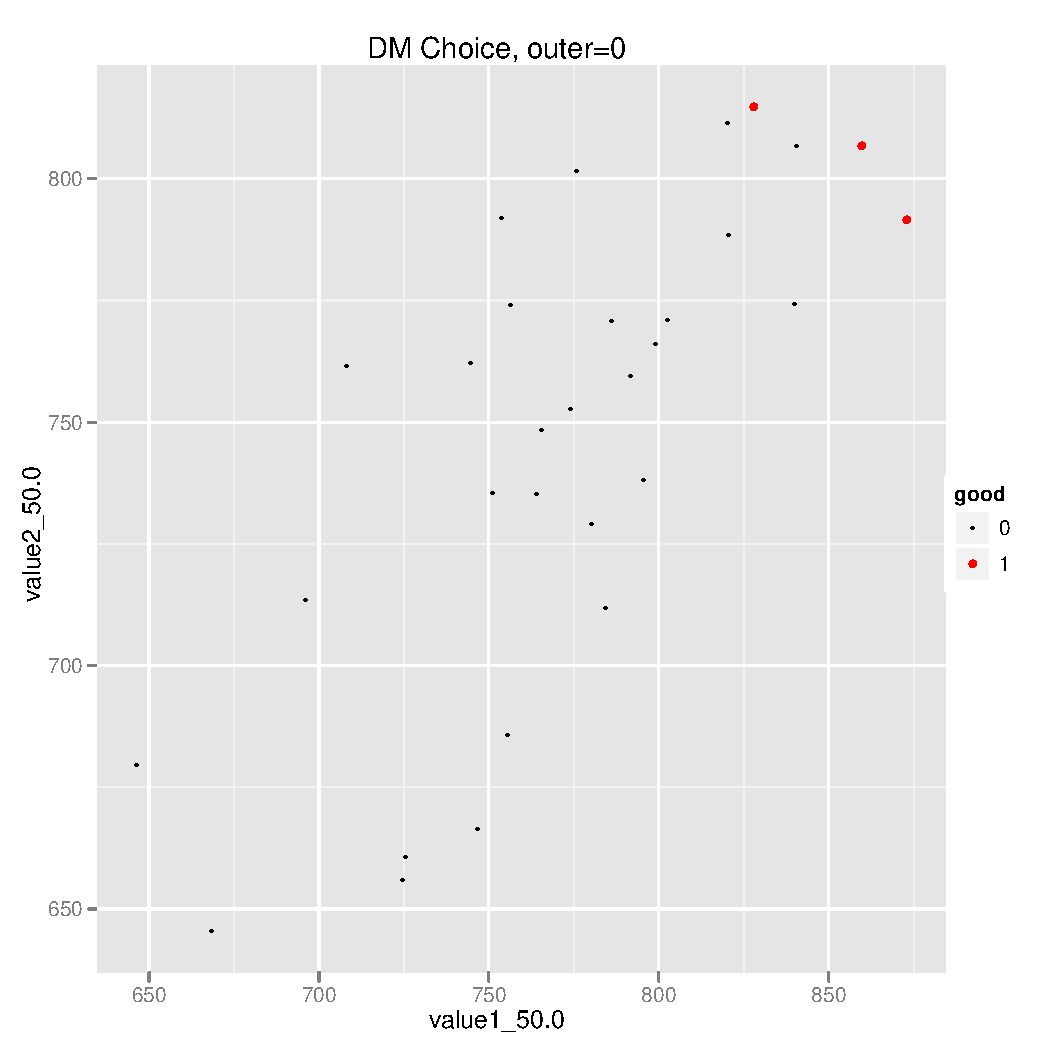
\includegraphics[scale=0.57]{exp/nouncert/c2_dmchoices_01}
    \label{c2_dmchoices_01}
  }
  \subfigure{
    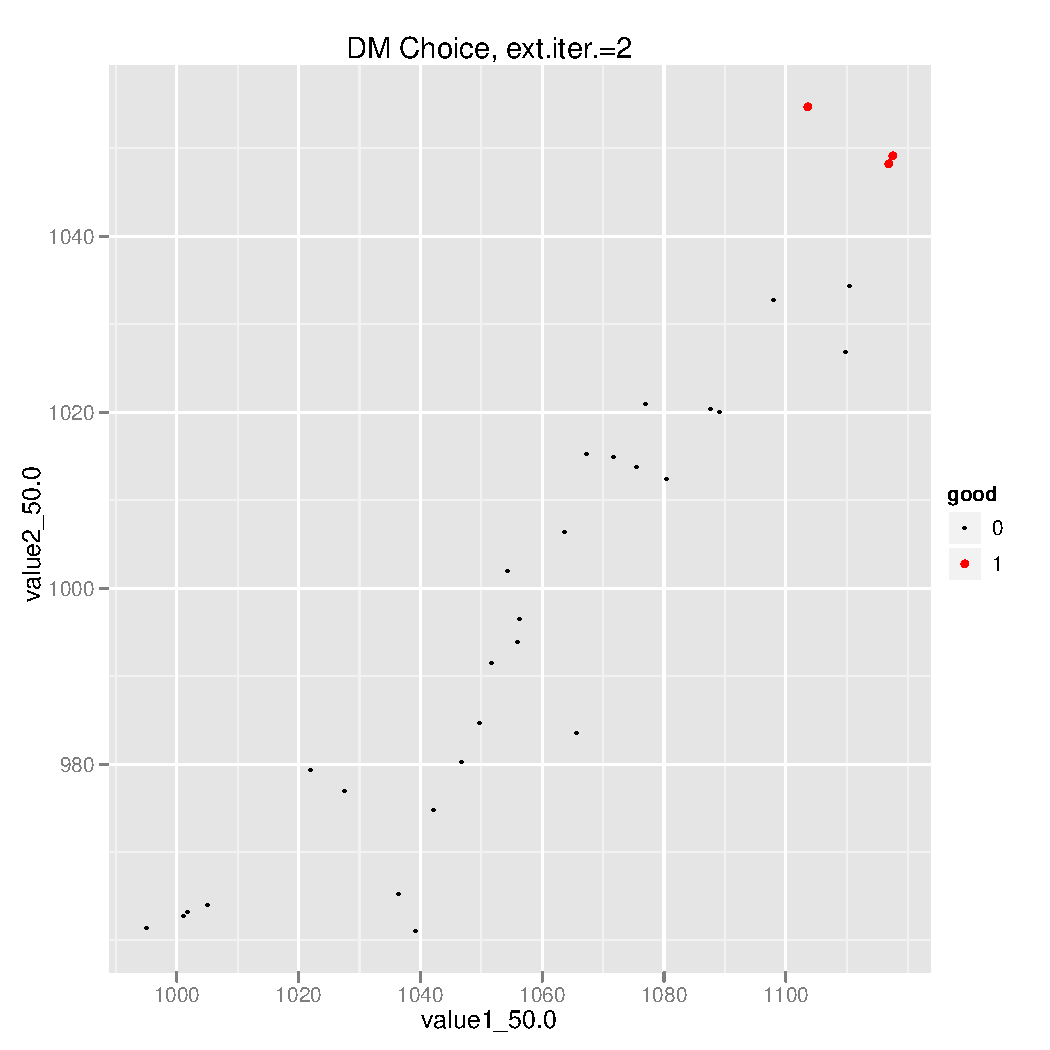
\includegraphics[scale=0.57]{exp/nouncert/c2_dmchoices_03}
    \label{c2_dmchoices_03}
  }
  \subfigure{
    \hspace*{2.5cm}
    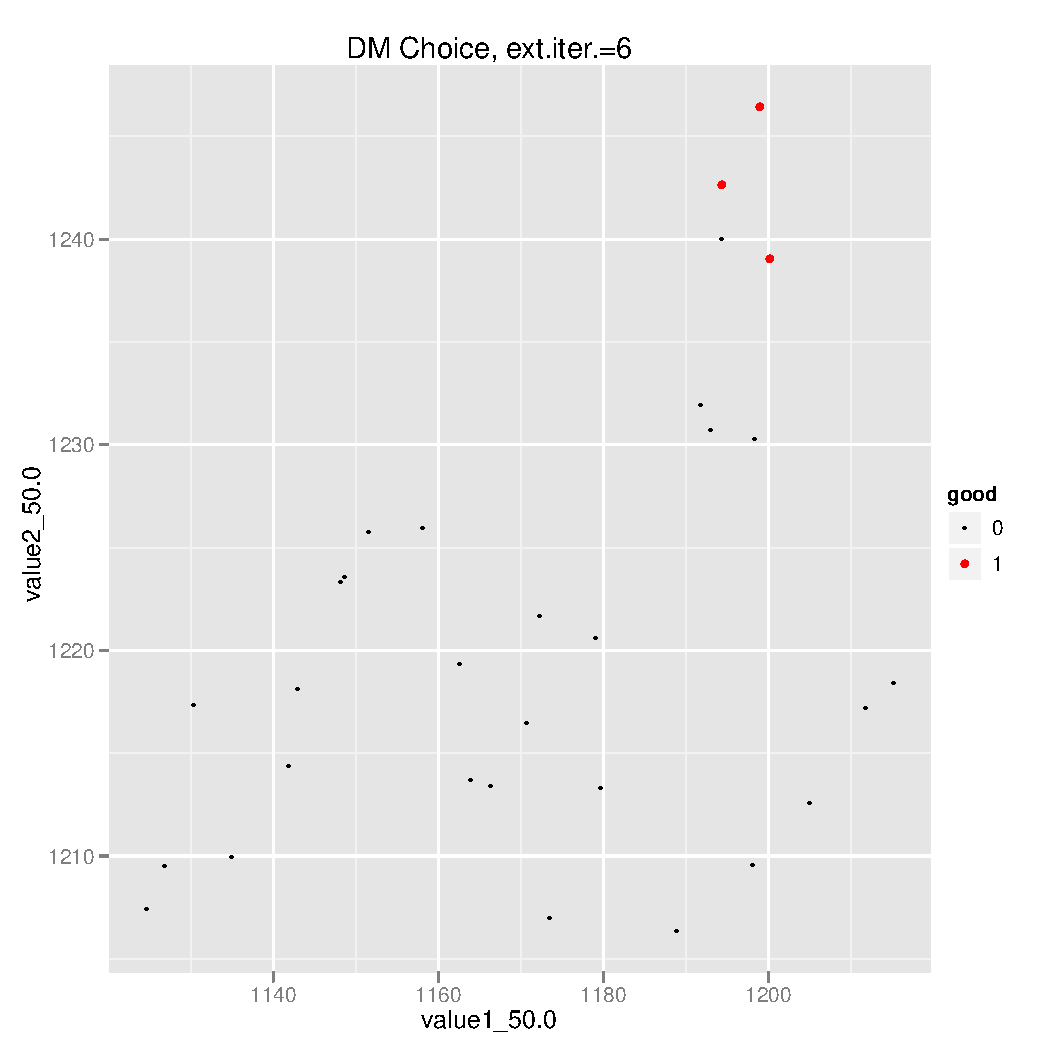
\includegraphics[scale=0.57]{exp/nouncert/c2_dmchoices_07}
    \label{c2_dmchoices_07}
  }
  \caption{Choices made by the DM in exterior loop}
\end{figure}


%% Utilind
\begin{figure}
  \centering 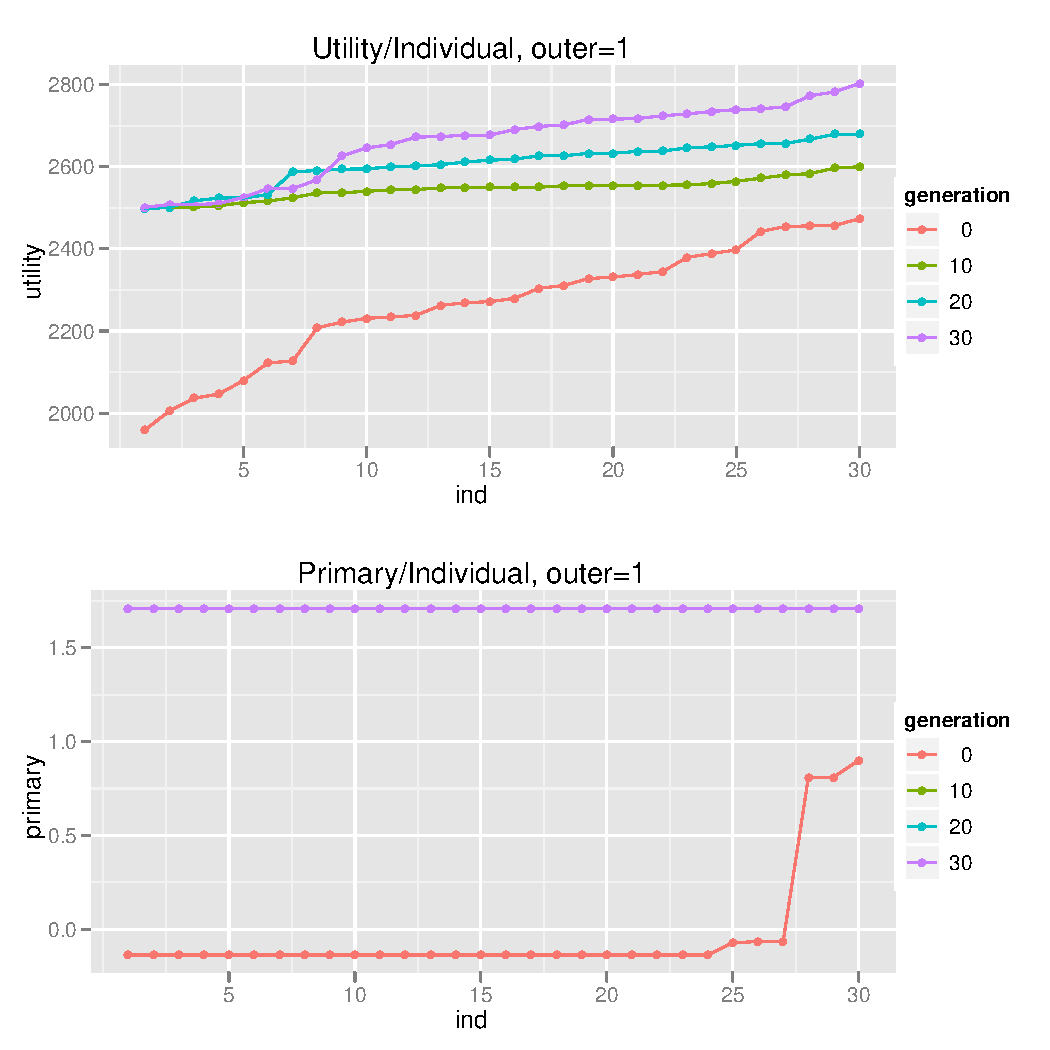
\includegraphics[width=1.0\textwidth]{exp/nouncert/c2_utilind_01}
  \caption{Population advancing through the generations of interior loop}
  \label{c2_utilind_01}
\end{figure}

\begin{figure}
  \centering 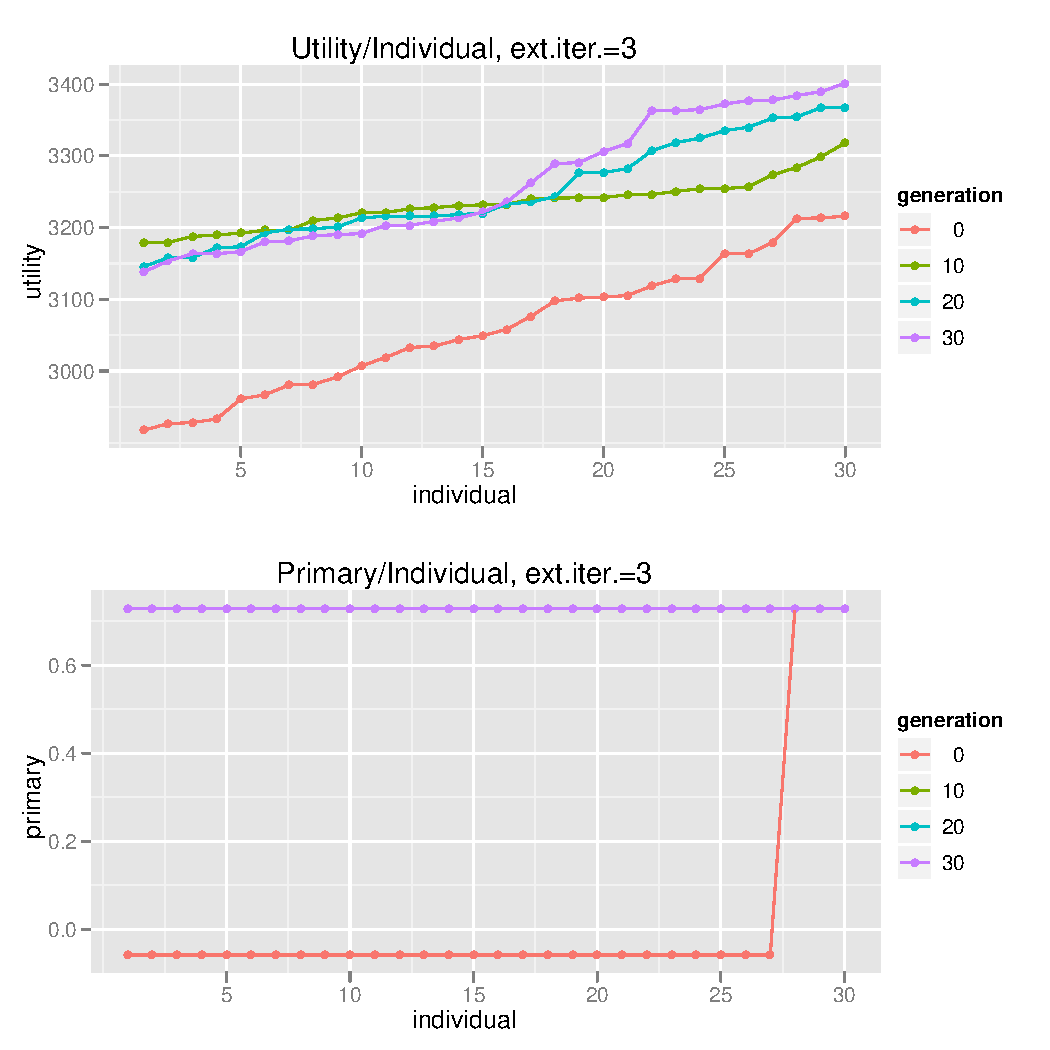
\includegraphics[width=1.0\textwidth]{exp/nouncert/c2_utilind_03}
  \caption{Population advancing through the generations of interior loop}
  \label{c2_utilind_03}
\end{figure}

\begin{figure}
  \centering 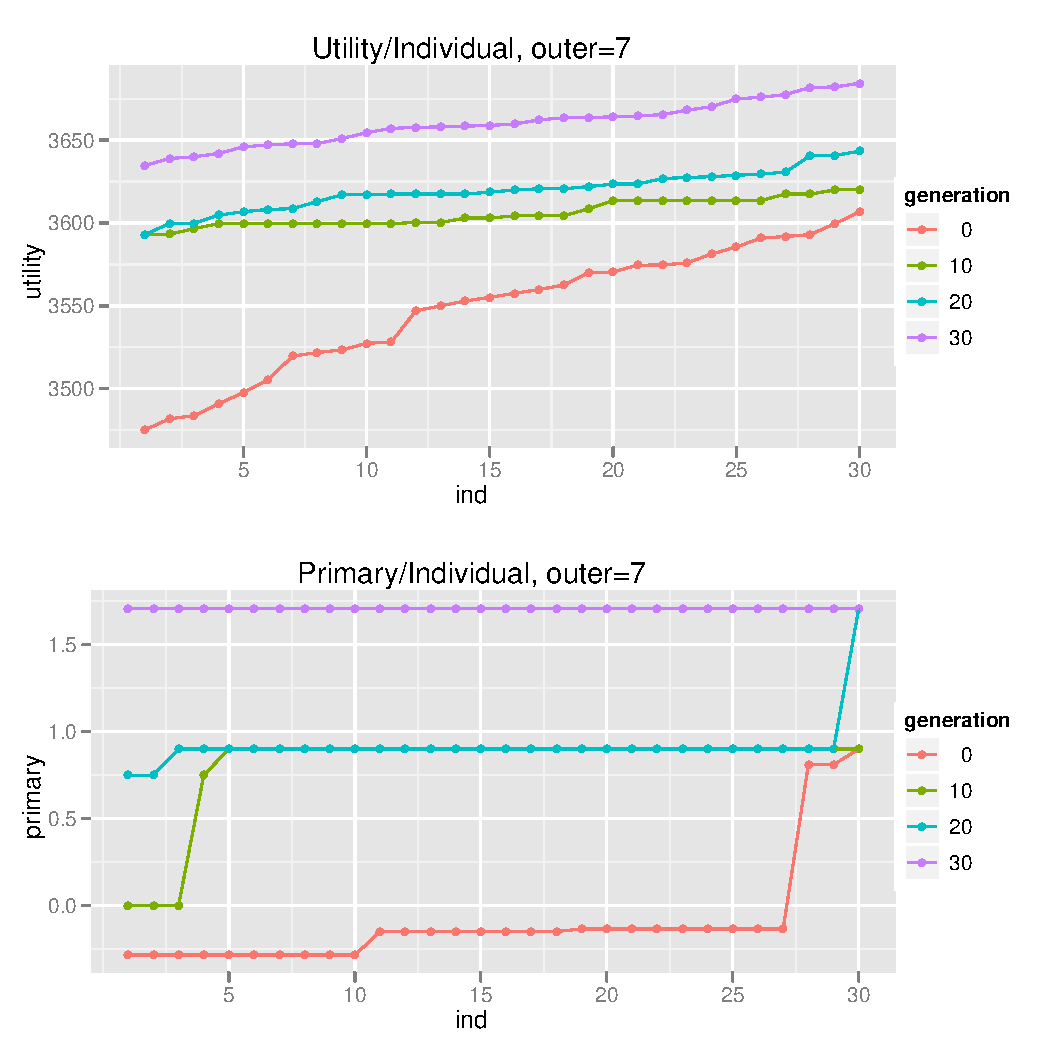
\includegraphics[width=1.0\textwidth]{exp/nouncert/c2_utilind_07}
  \caption{Population advancing through the generations of interior loop}
  \label{c2_utilind_07}
\end{figure}


\clearpage{}
\subsection{The performance on exemplary problems}
It is important to know what performance can be expected from an
algorithm. When no uncertainty is considered in a problem and one assumes
supposed utility function is easy to get optimal solution using linear
programming solver. Of course in real-world applications supposed utility
function is not known a priori. One can test this algorithm in such an
artificially created environment and then assume that the behaviour will be
similar on similar real-world problems.

Results of the evaluation on the following problems are given (see~[inref]):
\begin{itemize}
\item Two-criteria binary knapsack problem, optimal value $= 4154.441453$.
\item Two-criteria continuous knapsack problem, optimal value $= 32700.41689$.
\item Three-criteria binary knapsack problem, optimal value $= 31502.10927$.
\item Three-criteria DTLZ problem generated using constraint surface approach, optimal value $= -1.1$.
\end{itemize}

The test were repeated at least fifteen times and the results averaged. They
are presented on figure~\ref{simple_performance}. Depending on a problem $10$
or $20$ iterations of exterior loop were simulated. Normally it would be up to
the DM to stop when he or she is satisfied with the solution. However one can
safely assume that if no satisfactory solution is found in $10$ the decision
maker will not want to investigate the problem with this method further.

\begin{figure}
  \subfigure{
    \hspace*{-3.5cm}
    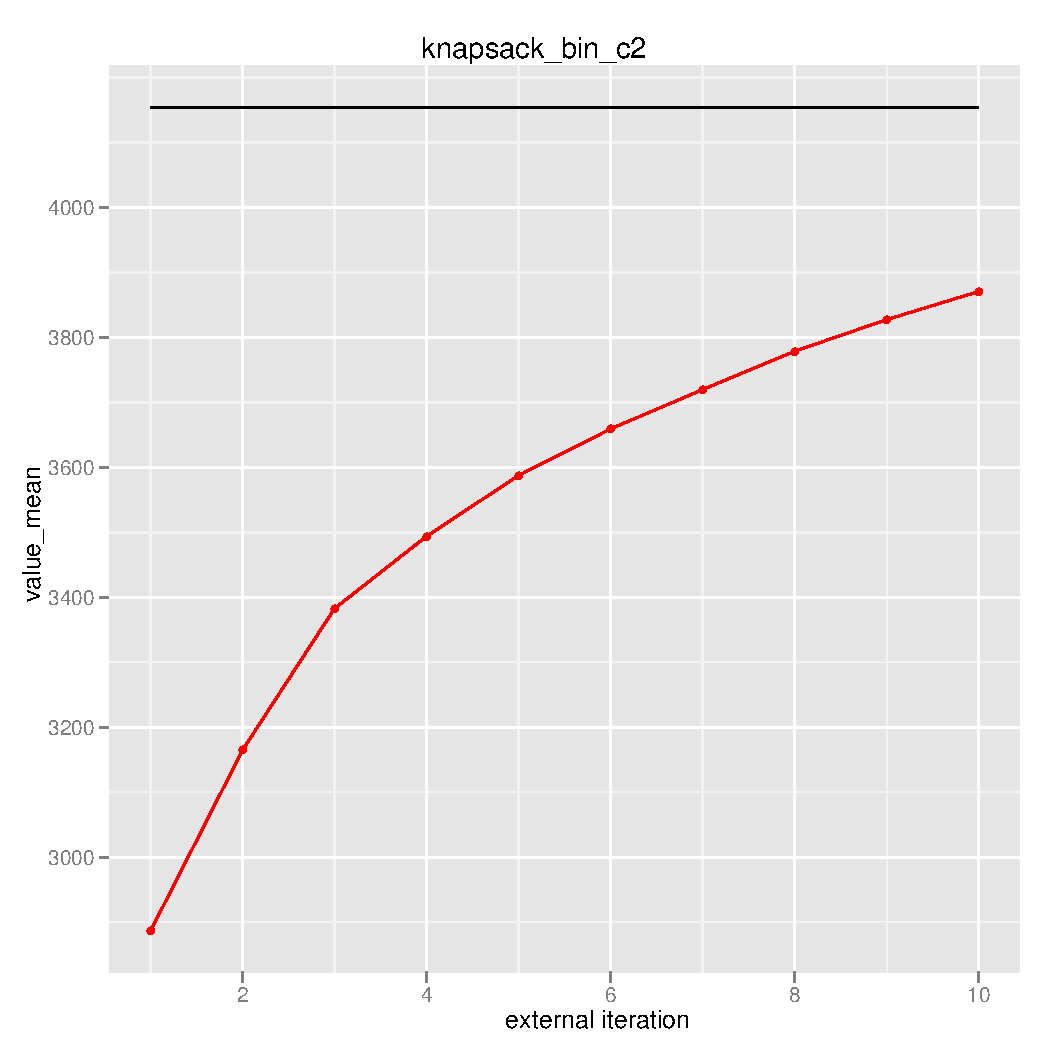
\includegraphics[scale=0.57]{exp/nouncert/c2_knapsack_bin}
    \label{simple_performance1}
  }
  \subfigure{
    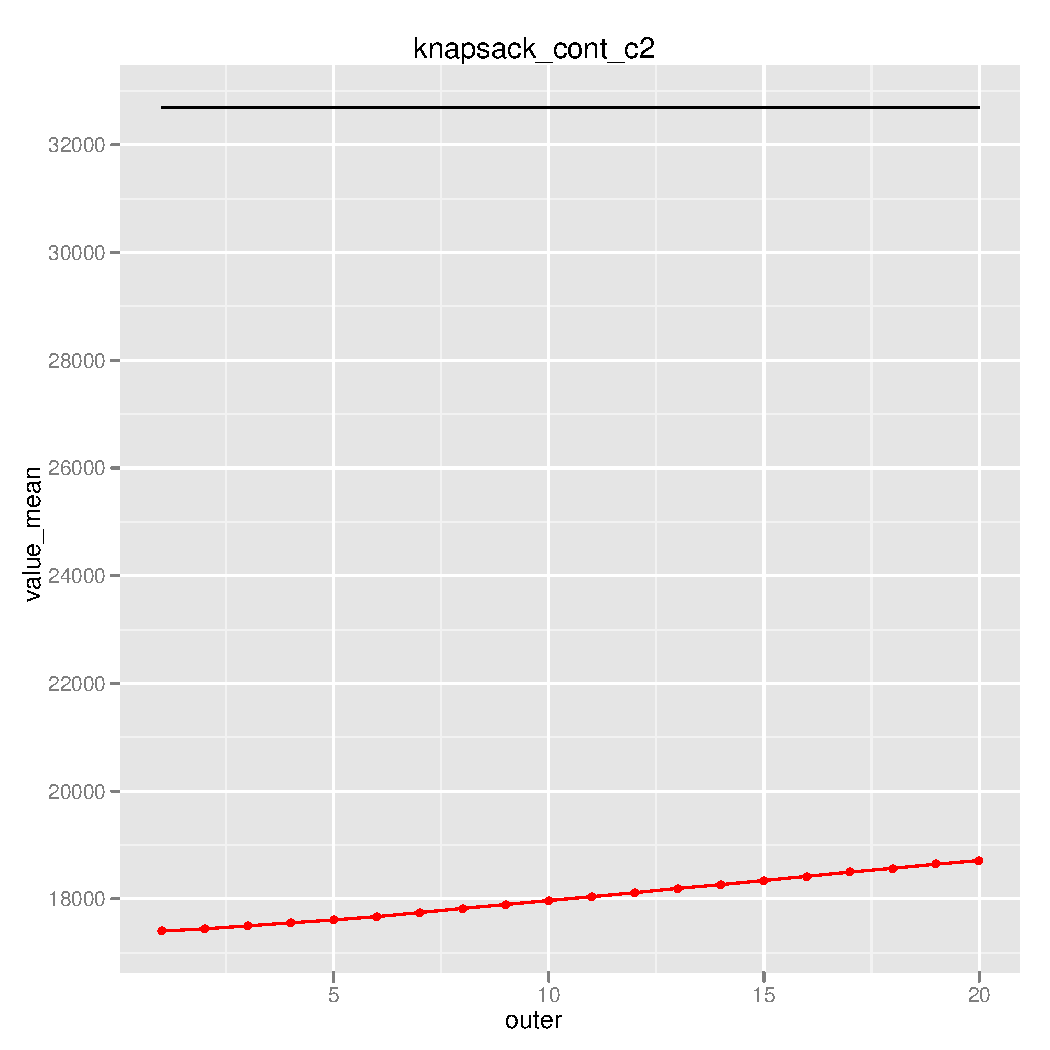
\includegraphics[scale=0.57]{exp/nouncert/c2_knapsack_cont}
    \label{simple_performance2}
  }
  \subfigure{
    \hspace*{-3.5cm}
    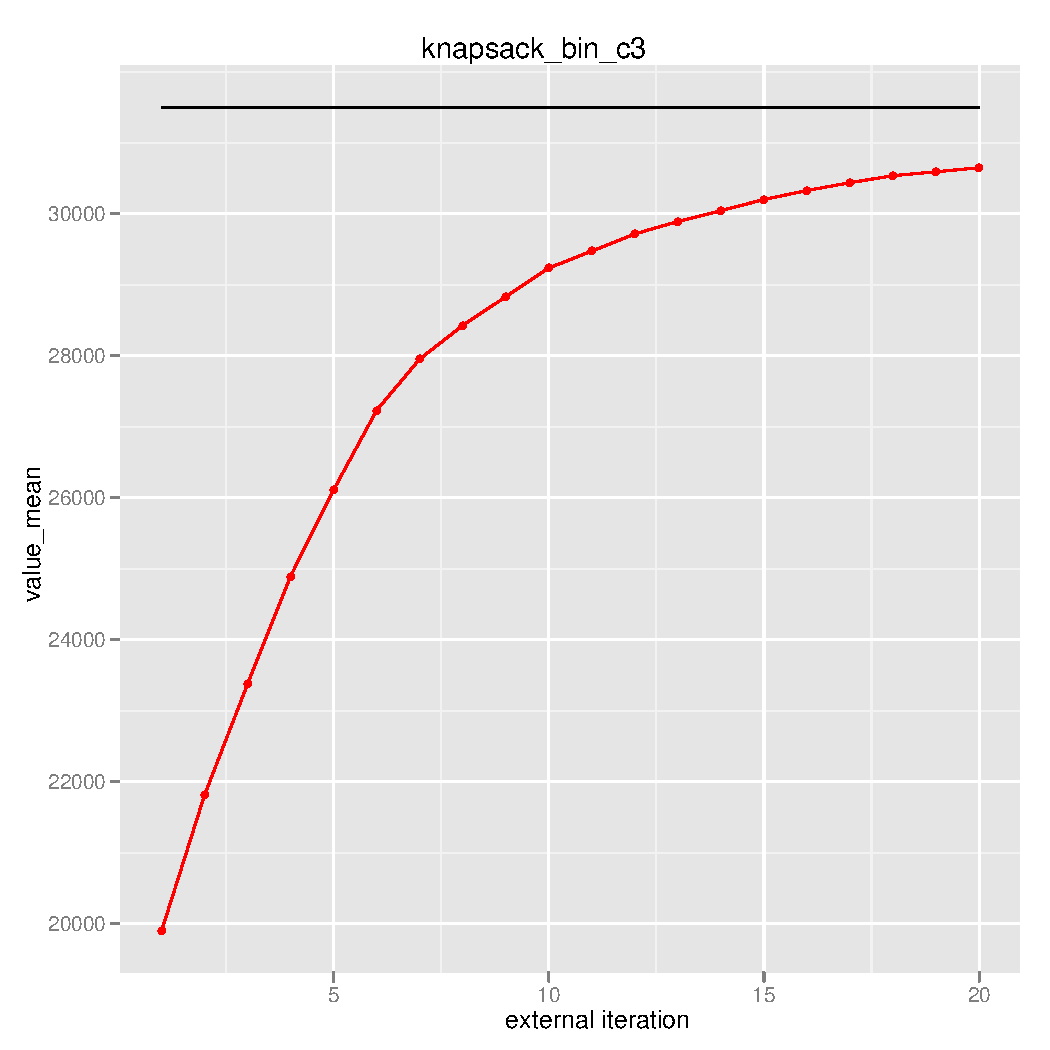
\includegraphics[scale=0.57]{exp/nouncert/c3_knapsack_bin}
    \label{simple_performance3}
  }
  \subfigure{
    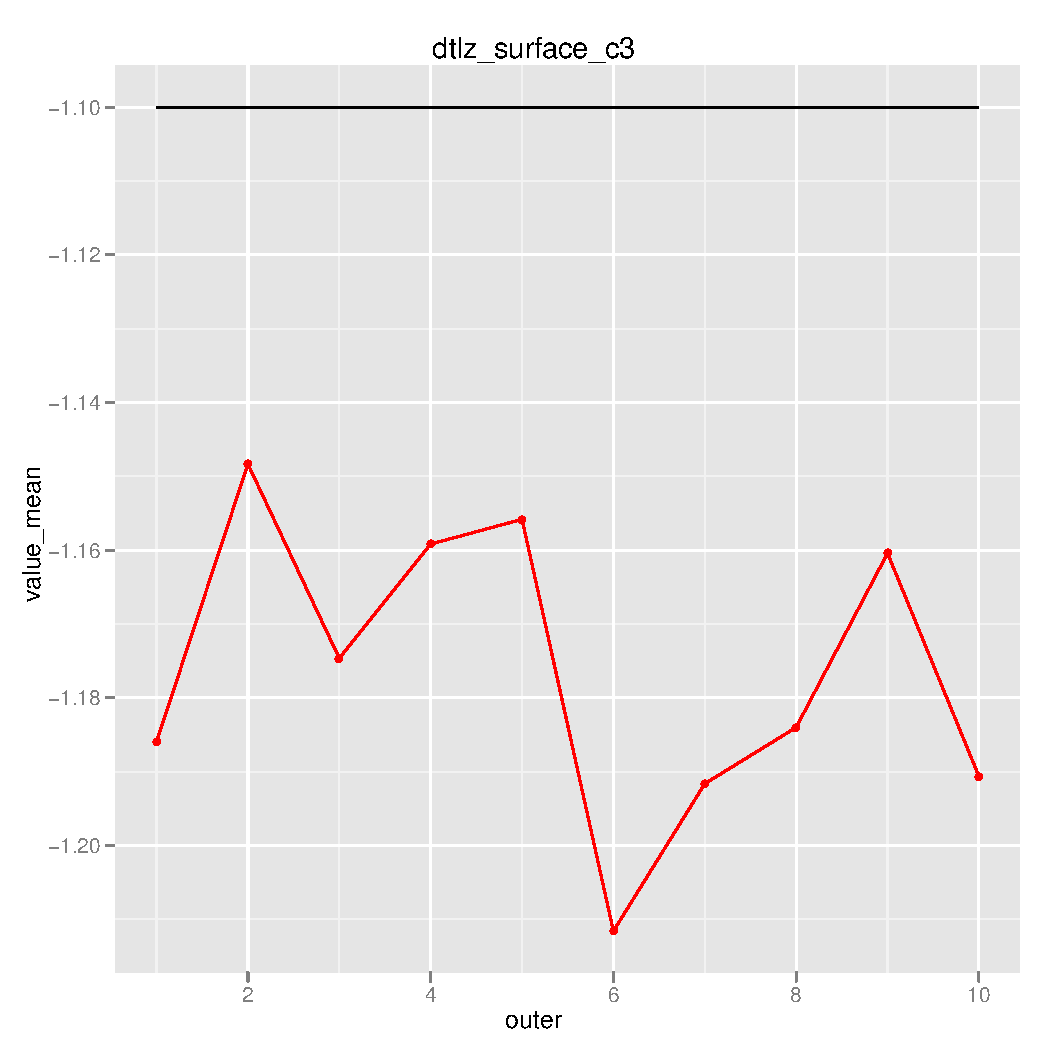
\includegraphics[scale=0.57]{exp/nouncert/c3_surface}
    \label{simple_performance4}
  }
  \caption{Performance comparison}
  \label{simple_performance}
\end{figure}

On both binary knapsack problems the performance is very good --- they are not
further than $10\%$ away from optimal solution after $10^{th}$ iteration. The
same is true for the surface problem. However looking at the
fig.~\ref{simple_performance4} one can see a bizarre phenomenon --- the
supposed utility is falling down in a few runs.

On the other hand evolutionary algorithm knows nothing about the utility
function so it may happen. The chart (fig.~\ref{simple_performance4}) was
generated using aggregated (averaged) results, however this happened in most
of the runs. To give further insight charts showing evolution in a third
exterior loop are presented (not that the charts are for single run only, not
aggregated). The charts are on figures~\ref{c3_surface_utilgen_03}
and~\ref{c3_surface_utilind_03}. As one can see the evolutionary algorithm
improves the population from its perspective (the primary score factor)
however supposed utility function is being lowered in the process.

\begin{figure}
  \centering
  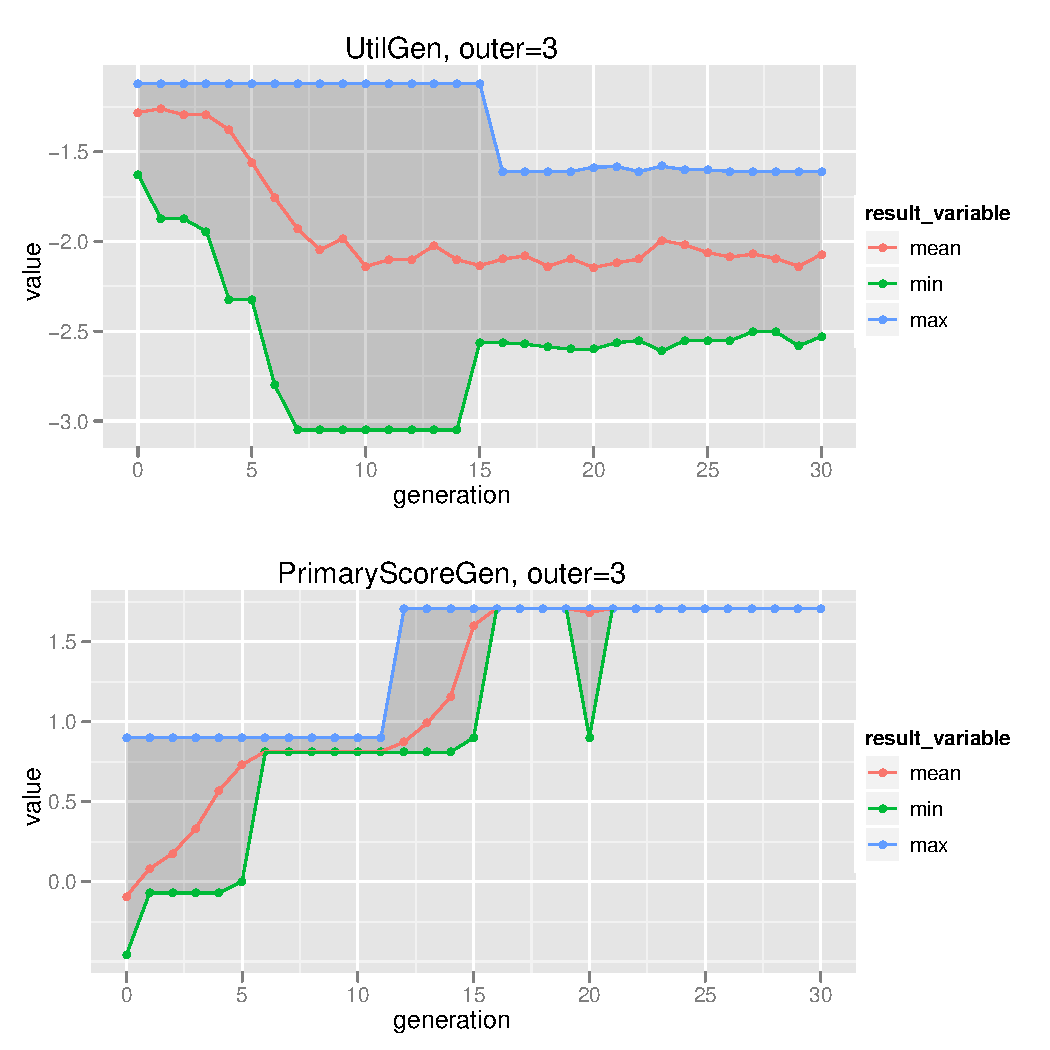
\includegraphics[width=1.0\textwidth]{exp/nouncert/c3_surface_utilgen_03}
  \caption{The population in the third iteration of the exterior loop. DTLZ
    surface problem.}
  \label{c3_surface_utilgen_03}
\end{figure}

\begin{figure}
  \centering
  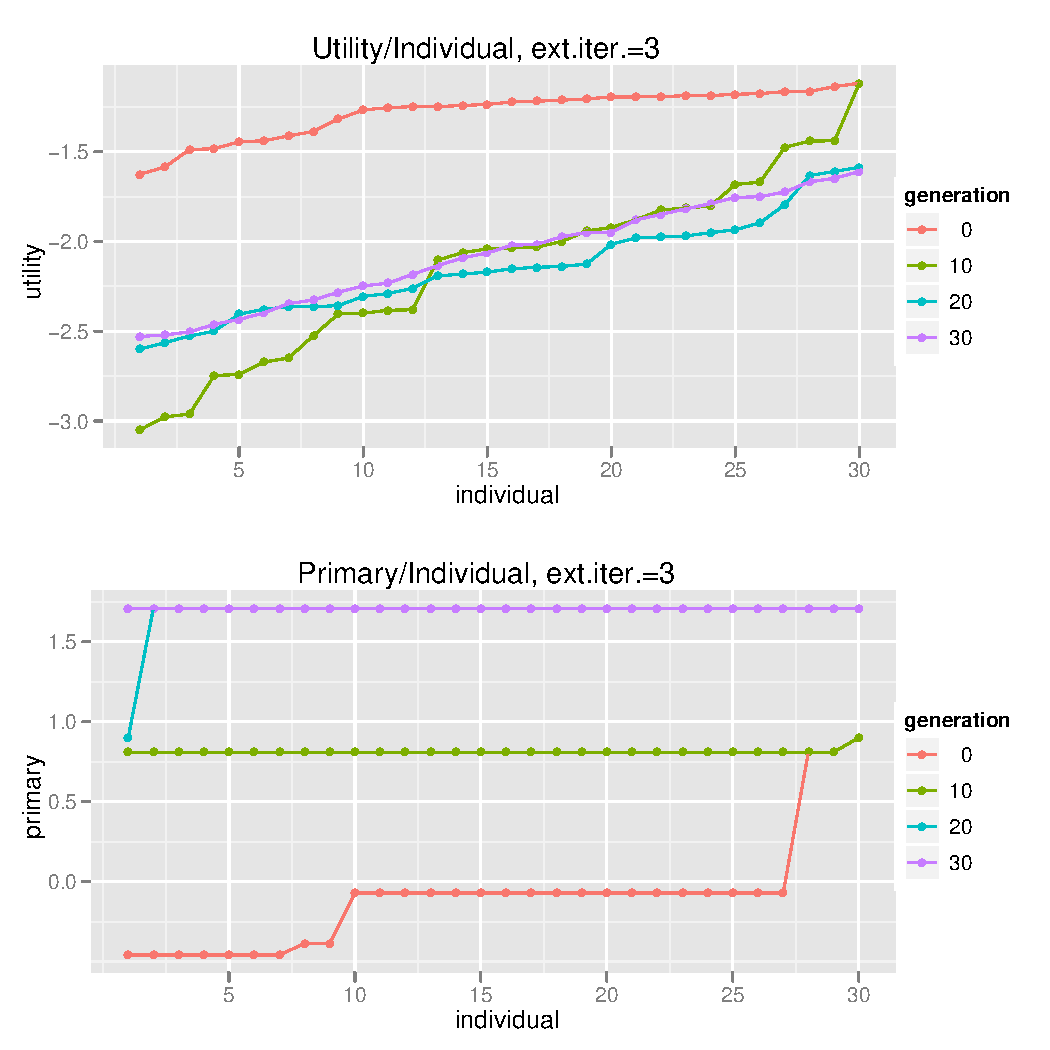
\includegraphics[width=1.0\textwidth]{exp/nouncert/c3_surface_utilind_03}
  \caption{The population in the third iteration of the exterior loop. DTLZ
    surface problem}
  \label{c3_surface_utilind_03}
\end{figure}

This is the case because generated decision rules:
\begin{enumerate}
\item $f_1 \le 0.14033 \Rightarrow \text{class} \ge \texttt{GOOD}$
\item $f_3 \le 0.56462 \Rightarrow \text{class} \ge \texttt{GOOD}$
\end{enumerate}
are not selective enough. It is possible than switching DomLem to another
algorithm, generating all possible rules instead of minimal set would help
here. Still the results achieved by the DARWIN method are good on this
problem.

In contrary continuous knapsack problem performs extremely poor --- only
$55\%$ of the optimum after $10^{th}$ run and $58\%$, so almost no
improvement, after $20^{th}$. Investigating single runs in details provided no
more details. The problem lies in the evolutionary algorithm, more precisely
in its crossover operator. Authors suggested a from of distance preserving
crossover --- child is somewhere in between its parents. However in continuous
it is usually the case to take items one-by-one starting with the one with
greatest value per unit until the weight constraint is reached.

Considering the constraints ($ \forall_{x_i \in items}: \hspace{0.1cm} 0 \leq
x_i \leq 1 $) --- most of the individuals will have its decision variables in
form of $x_i \approx 0.5$ after a few generations. But for the optimal
solutions most of the variables takes either $1$ or $0$. That is why
improvement is happening so slowly here.

According to authors intuition changing the crossover operator would solve the
problem with continuous knapsack. Choosing the right operator for a given
problem is a well-known subject in the multi-objective optimisation
([ref]). However it is out-of-scope of this paper.

For completeness charts presenting the algorithm behaviour when more exterior
loop iterations are allowed are given (fig.~\ref{outer}). After the twentieth
loop improvements are small (if any). In author's opinion this is a good thing
because there is no reason not to stop algorithm. If it works for the problem
it will be evident from the first few iterations.

\begin{figure}
  \subfigure{
    \hspace*{-2.5cm}
    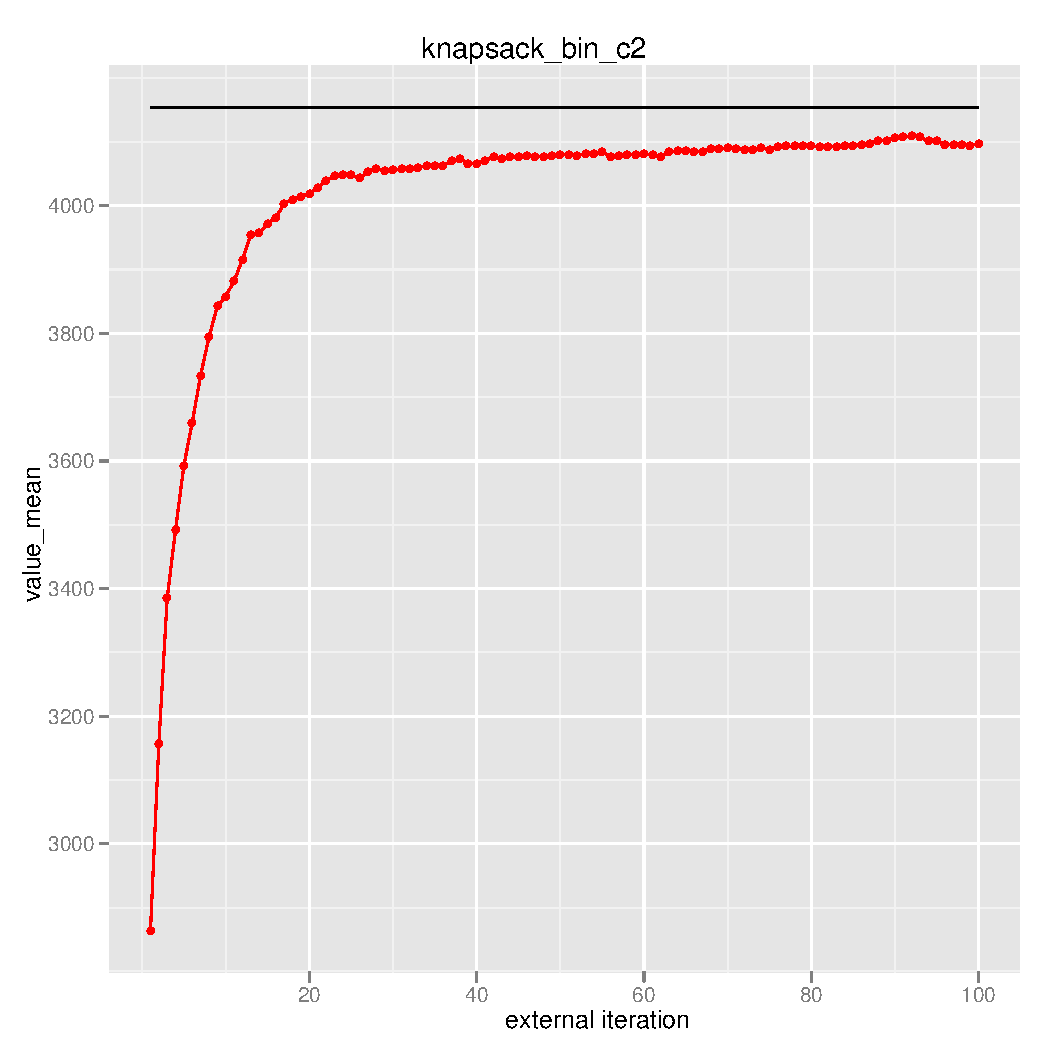
\includegraphics[scale=0.57]{exp/nouncert/c2_knapsack_bin_outer}
    \label{outer1}
  }
  \subfigure[TODO!]{
    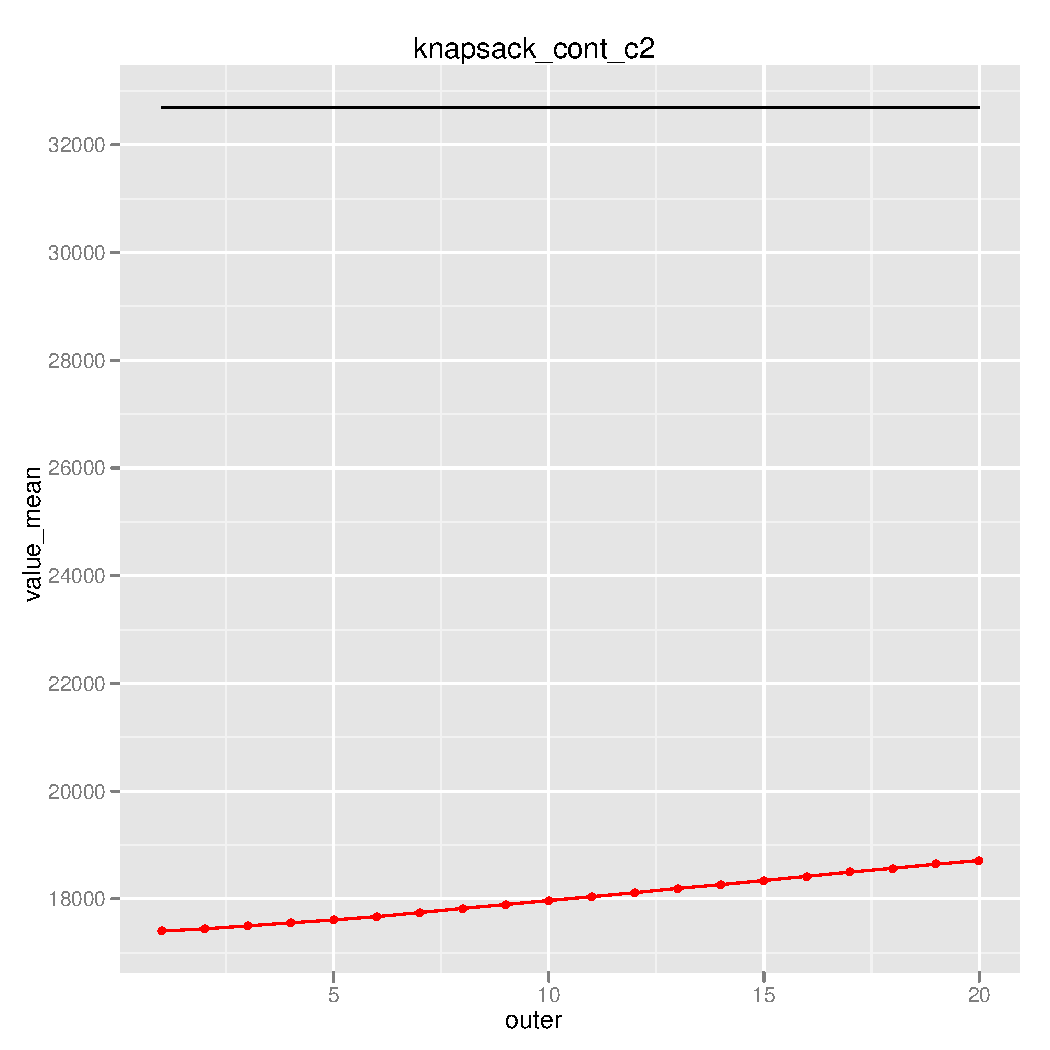
\includegraphics[scale=0.57]{exp/nouncert/c2_knapsack_cont}
    \label{outer2}
  }
  \subfigure{
    \hspace*{-2.5cm}
    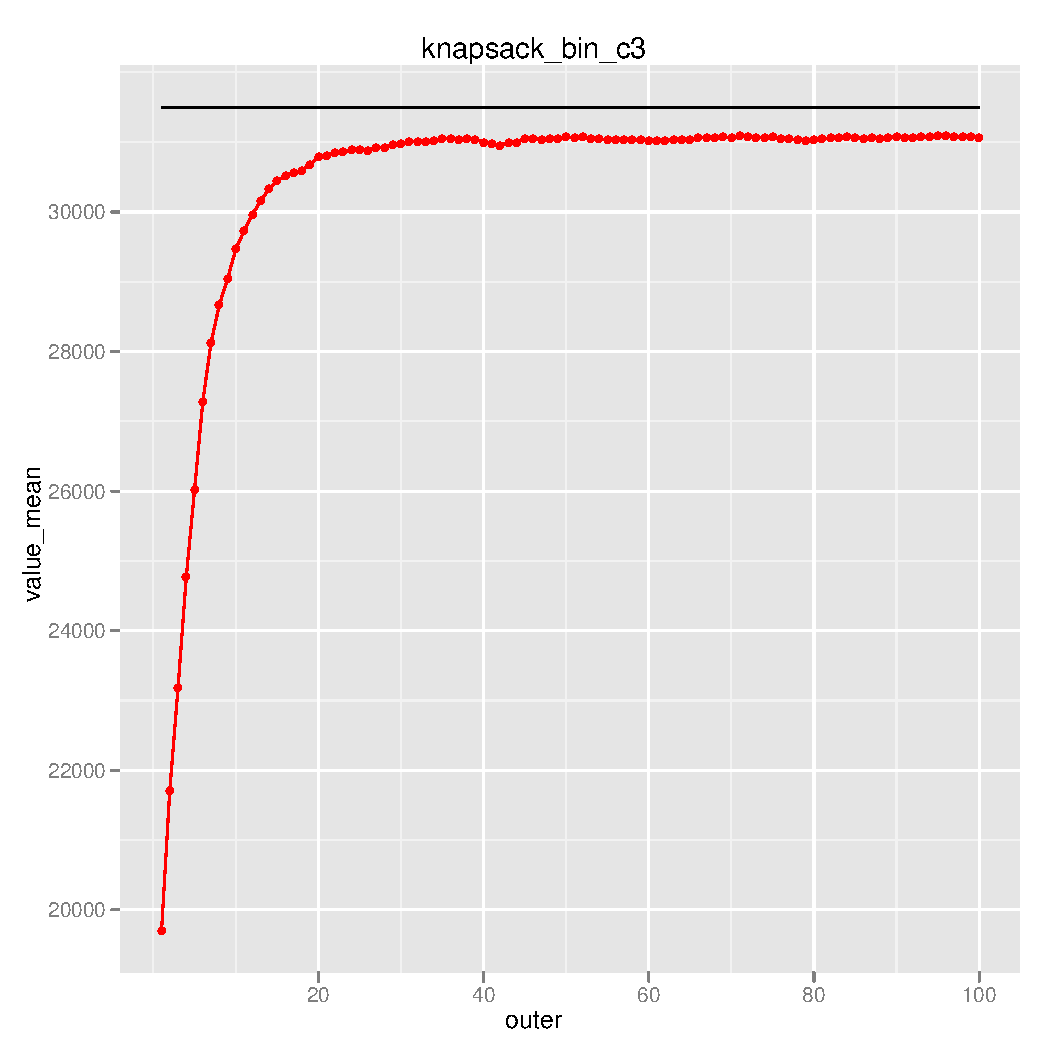
\includegraphics[scale=0.57]{exp/nouncert/c3_knapsack_bin_outer}
    \label{outer3}
  }
  \subfigure{
    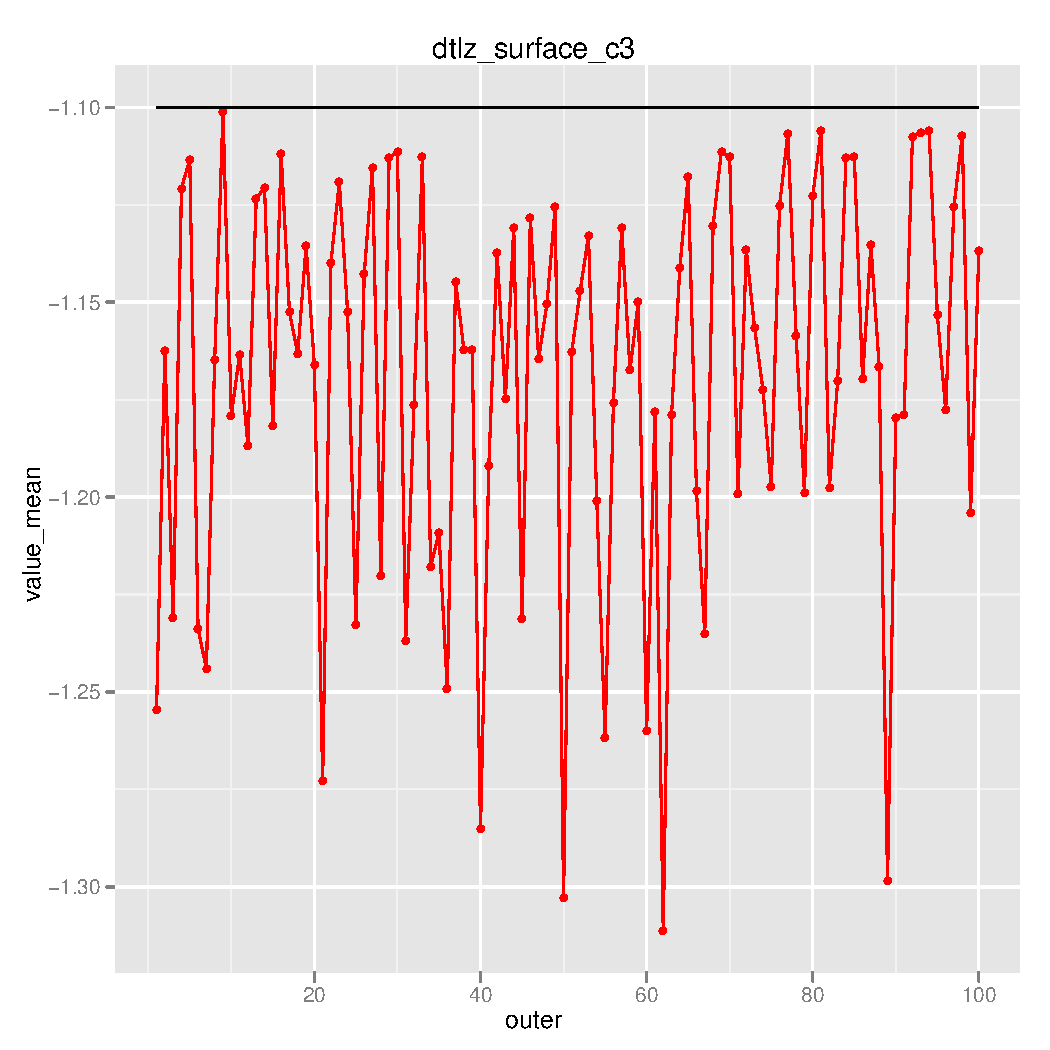
\includegraphics[scale=0.57]{exp/nouncert/c3_surface_outer}
    \label{outer4}
  }
  \caption{Supposed utility function when long runs are allowed}
  \label{outer}
\end{figure}



\clearpage{}
\section{The importance of parameters}

The algorithm itself contains many parameters that can potentially affect its
behaviour. Of course it is always left to analyst to fine-tune the parameters
for a specific problem to solve. Nevertheless in this section some guidelines
will be given. Conclusions were drawn based on experiments performed on
exemplary problems described above.

The parameters were grouped into two categories --- basic ones affecting the
whole method and additional ones of less importance. The latter however can be
used for fine-tuning to specific problem given.

Author consider basic parameters to be:
\begin{itemize}
\item Number of generation in the evolutionary loop --- intuitively the more
  the better.
\item Number of individuals in the population --- again intuitively the more
  the better.
\item A confidence of the rules generated in the DomLem algorithm. (compare
  with~[inref]). 100\% confidence may seem a good idea however lowering it
  would allow more gradual improvements of the goal function in the
  evolutionary algorithm which could lead to better results.
\end{itemize}



\clearpage{}
\section{Noise in the DM's decisions}

\section{Uncertainty}

\section{Conclusions}

